\documentclass[12pt]{article}

\usepackage[utf8]{inputenc}
\usepackage{fancyhdr} % Required for custom headers
\usepackage{lastpage} % Required to determine the last page for the footer
\usepackage{extramarks} % Required for headers and footers
\usepackage[usenames,dvipsnames]{color} % Required for custom colors
\usepackage{graphicx} % Required to insert images
\usepackage{listings} % Required for insertion of code
\usepackage{courier} % Required for the courier font
\usepackage{lipsum} % Used for inserting dummy 'Lorem ipsum' text into the template
\usepackage{hyperref}
\usepackage{dirtree}

% Margins
%\topmargin=-0.45in
%\evensidemargin=0in
%\oddsidemargin=0in
%\textwidth=6.5in
%\textheight=9.0in
%\headsep=0.25in

\topmargin 0.0cm
\oddsidemargin 0.2cm
\textwidth 16cm 
\textheight 21cm
\footskip 1.0cm

\linespread{1.2} % Line spacing

% Set up the header and footer
\pagestyle{fancy}
\lhead{Tomas Rojo} % Top left header
%\chead{}
\rhead{Music Information Retrieval and Genre Classification} % Top right header
%\lfoot{}
%\cfoot{}
%\rfoot{}
\renewcommand\headrulewidth{0.4pt} % Size of the header rule
\renewcommand\footrulewidth{0.4pt} % Size of the footer rule

%\setlength\parindent{0pt} % Removes all indentation from paragraphs

%----------------------------------------------------------------------------------------
%	CODE INCLUSION CONFIGURATION
%----------------------------------------------------------------------------------------

\definecolor{codegreen}{rgb}{0,0.6,0}
\definecolor{codegray}{rgb}{0.5,0.5,0.5}
\definecolor{codepurple}{rgb}{0.58,0,0.82}
\definecolor{backcolour}{rgb}{0.95,0.95,0.92}
\lstloadlanguages{Python}
\lstset{
	language=Python,
    backgroundcolor=\color{backcolour},   
    commentstyle=\color{codegreen},
    keywordstyle=\color{magenta},
    numberstyle=\tiny\color{codegray},
    stringstyle=\color{codepurple},
    basicstyle=\footnotesize,
    breakatwhitespace=false,         
    breaklines=true,                 
    captionpos=b,                    
    keepspaces=true,                 
    numbers=left,                    
    numbersep=5pt,                  
    showspaces=false,                
    showstringspaces=false,
    showtabs=false,                  
    tabsize=2
}

% Creates a new command to include python
\newcommand{\pyscript}[2]{
\begin{itemize}
\item[]\lstinputlisting[caption=#2,label=#1]{#1.py}
\end{itemize}
}

%----------------------------------------------------------------------------------------
%	TITLE PAGE
%----------------------------------------------------------------------------------------

\title{\textbf{Music Information Retrieval and Genre Classification} }
\author{Tomas Rojo}
\date{} % Insert date here if you want it to appear below your name


%----------------------------------------------------------------------------------------

\begin{document}

% Double-space the manuscript.

\baselineskip8pt

% Make the title.

\maketitle 

%----------------------------------------------------------------------------------------
%	TABLE OF CONTENTS
%----------------------------------------------------------------------------------------

%\setcounter{tocdepth}{1} % Uncomment this line if you don't want subsections listed in the ToC

%\newpage
%\tableofcontents
%\newpage

%----------------------------------------------------------------------------------------





%----------------------------------------------------------------------------------------

\section*{Introduction}

Machine Learning has been used extensively in the field of music. Both supervised and unsupervised learning techniques have been successfully applied for tasks such as genre classification, recommender systems, and clustering. However using music as input data is trickier than using other sets of data such as numeric vectors of expenses, for example. The first step in implementing Machine Learning systems for music is to treat our input data, music, in a way that the machine can understand.
\medskip

This report offers an overview of the ideas and techniques that are commonly used in the field of Music Information Retrieval, as well as an exploration of musical genre classification using machine learning techniques. The code accompanying this report is intended for readers to follow along and explore this fascinating field by providing ways to import and play with the reader's own mp3 library.
\medskip

We begin by asking the most basic question: what is sound and how can we translate it into machine-understandable language. Once we have built our dataset we will explore a common application of machine learning models to music: musical genre classification.
\medskip

The reader is referred to Apendix A for all necessary information on the python modules and programs required to follow along.
 

\section*{What is sound?}
Before we can turn music into something the computer can understand, we need to study what sound is. Sound is just a pressure wave, which means it is a disturbance of the atmospheric pressure that travels to our ears. This pressure wave has a series of characteristics that are important when transforming into machine language. These are: amplitude and frequency. The amplitude tells us how much air is being moved by the pressure wave, and translates to volume. The frequency tells us how quickly the wave oscillates and translates to pitch. A pure tone playing an A would vibrate 440 times per second in a sinusoidal manner, and would consist of a single frequency. A violin playing the same note, however, contains many other frequency components, known as harmonics, which when added up together make the timbre of the instrument. Because these harmonics interact and interfere with each other, a violin, or any other instrument playing a single note will not produce a purely sinusoidal wave. 
\medskip

A microphone picks up these pressure vibrations and translates them into an electrical current that replicates the shape, amplitudes and frequencies of sound. This current is then used, for example, to drive speakers which oscillate at those given parameters to reproduce sound.  Let's take a look at one of this waveforms. But before we do that we might as well take our first aside, and turn to code to convert our music libraries into wav files.

\subsection*{Converting your mp3 and m4a library to wav}

We begin by looking at the directory containing the music. It is advised that you store the music you want to convert in a structure  similar to this since we use the "genre" folder name to extract the genre as a label for supervised learning.

\medskip
	\begin{center}
    \begin{minipage}{0.5\textwidth}
    \end{minipage}%
    \begin{minipage}{0.5\textwidth}
    \medskip
    \dirtree{%
	.1 Main dir.
	.2 Genre 1.
	.3 Artist 1.
	.4 Album 1.
	.4 Album 2.
	.4 ....
	.3 Artist 2.
	.4 Album 1.
	.4 ....
	.3 ....
	.2 Genre 2.
	.3 Artist 1.
	.4 ....
	.3 ....
	.2 ....
	}
    \end{minipage}
	\end{center}

\medskip

Once the music has been organized, and after installing the necessary software as it appears on Appendix A, we can proceed to mass convert the selected media using the \textit{mass\_convert} function. Let's take a look at the first 20 seconds of three different tunes from three different genres: jazz, flamenco, and bluegrass, respectively:

\begin{figure}
\centering
  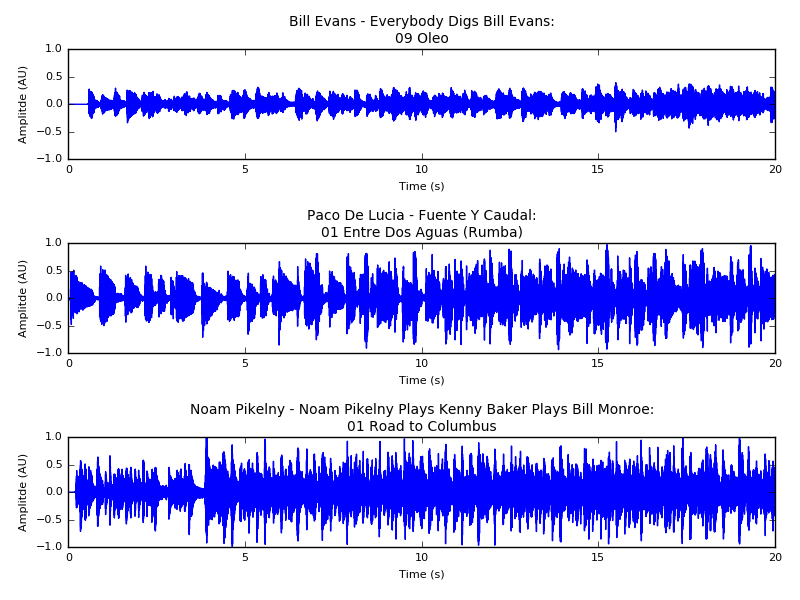
\includegraphics[width=0.75\textwidth]{waveforms.png}
  \caption{First 20 seconds of three different waveforms}
  \label{waveforms}
\end{figure}

\newpage

We see that pure waveforms are not readily informative. If shown these three different graphs separately it would be hard to tell which genre corresponds to which. One could naively consider feeding these waveforms directly into our machine learning models but that would be impractical: each of these waveforms is composed of millions of 2-byte integers!
\medskip

\section*{Music information retrieval}
\subsection*{Time domain features}
Instead we extract relevant and clever features from this waveform, dramatically reducing its dimensionality while still conveying information. One of this features is the \textbf{\textit{zero crossing rate}} or \textbf{\textit{ZCR}}. The \textit{ZCR} is a simple measure of the rate of change of the numbers of zero-crossings. It can be used to detect onsets, usually of percussive sounds and for monophonic sounds it can be used to estimate pitch, since the zero-crossings are related to frequency. It more generally describes the noisiness of a signal since noisy samples would have a higher zero crossing rate. 
\medskip

Figure \ref{zcr} shows the zero crossing rate for Paco de Lucia's "Entre dos aguas" song, which begins with a few solo notes on the bass. As we expect we see sharp peaks at the beginning of each bass note and then becomes a little bit harder to interpret. 
\medskip
\begin{figure}
\centering
  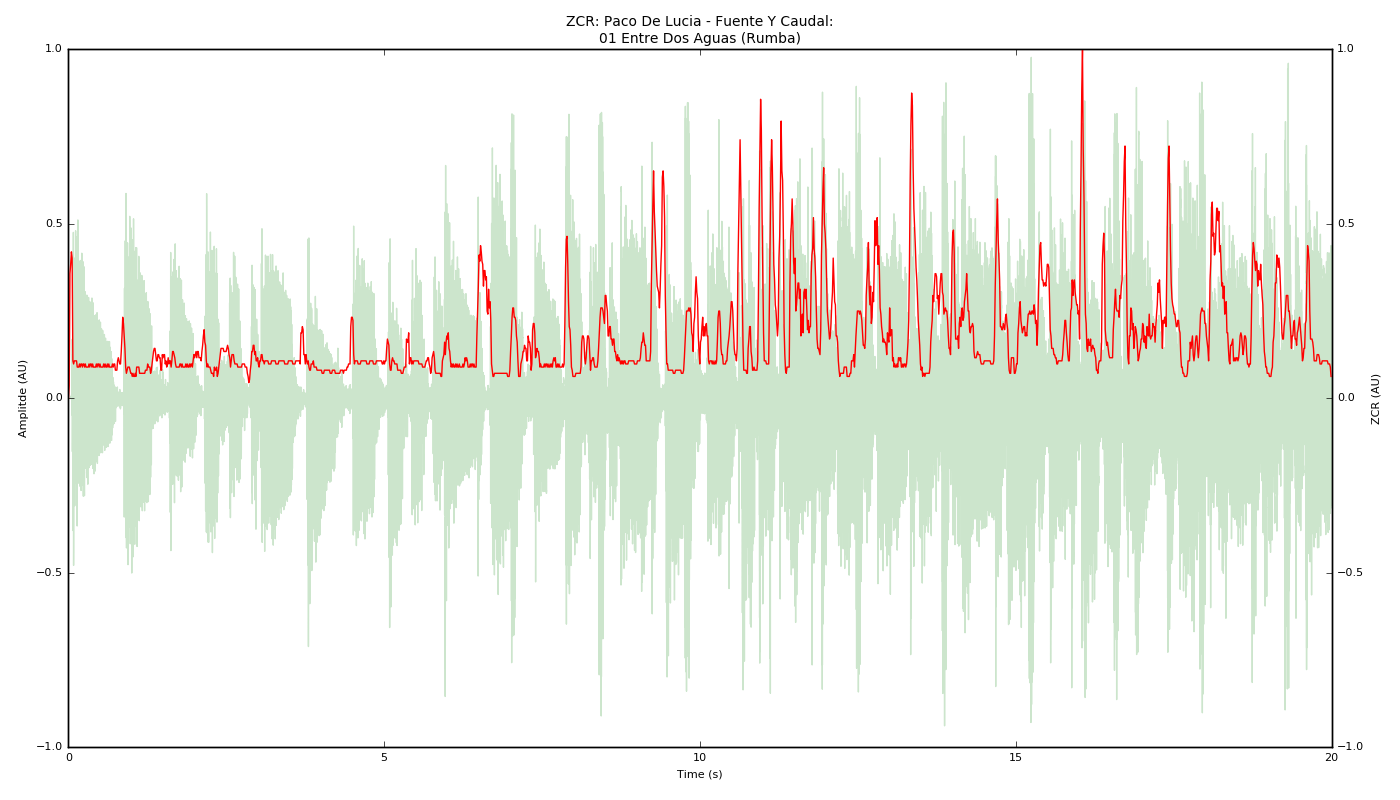
\includegraphics[width=0.75\textwidth]{ZCR_Entre_Dos_Aguas.png}
  \caption{ZCR superimposed on waveform for the first 20 seconds of a song}
  \label{zcr}
\end{figure}
\medskip

The next natural question to ask ourselves is whether there are substantial differences between the mean and standard deviation of this first feature across our genres. To do that we will pick three songs we consider representative of each genre and calculate the aforementioned quantities, as shown in fig \ref{zcr_genre}.
\begin{figure}
\centering
  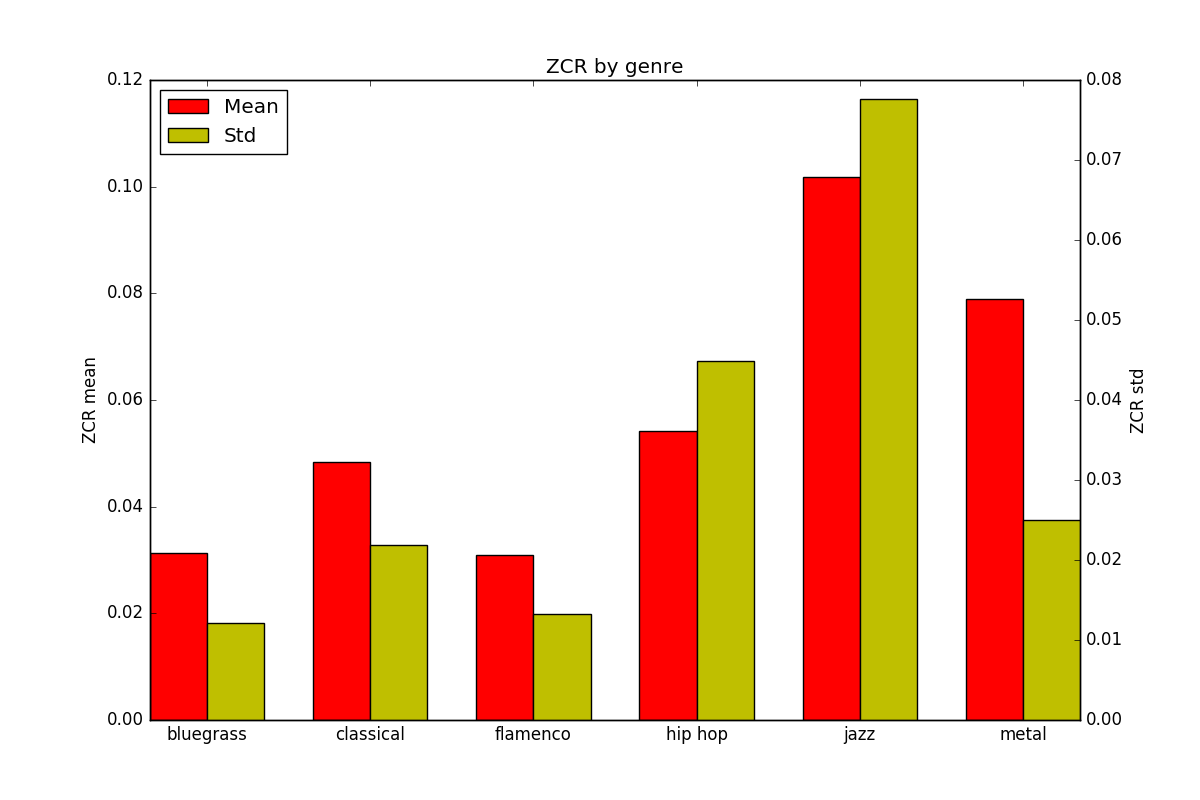
\includegraphics[width=0.75\textwidth]{ZCR_by_genre.png}
  \caption{Mean and std of ZCR across genres}
  \label{zcr_genre}
\end{figure}
\medskip

We see that there is enough difference between the values of the \textit{ZCR} among genres for this feature to be useful. It is very interesting to see that the values for flamenco and bluegrass are close to equal. This may be due to a coincidence since at first sight the two genres are very different. However from a wider perspective, flamenco and bluegrass are both folklorical genres based upon similar harmonic structures, and with similar harmonic content and a not too different instrumentation.
\medskip

The next feature we look at is the \textbf{\textit{Root mean square}} or \textbf{\textit{RMS}}. The \textit{RMS} is a measure of the wave's energy, and can be roughly translated into the overall loudness of the track. Once again, let's look at the \textit{RMS} for Paco de Lucia's tune, and how its mean and std vary across genres:
\medskip

\begin{figure}
\centering
  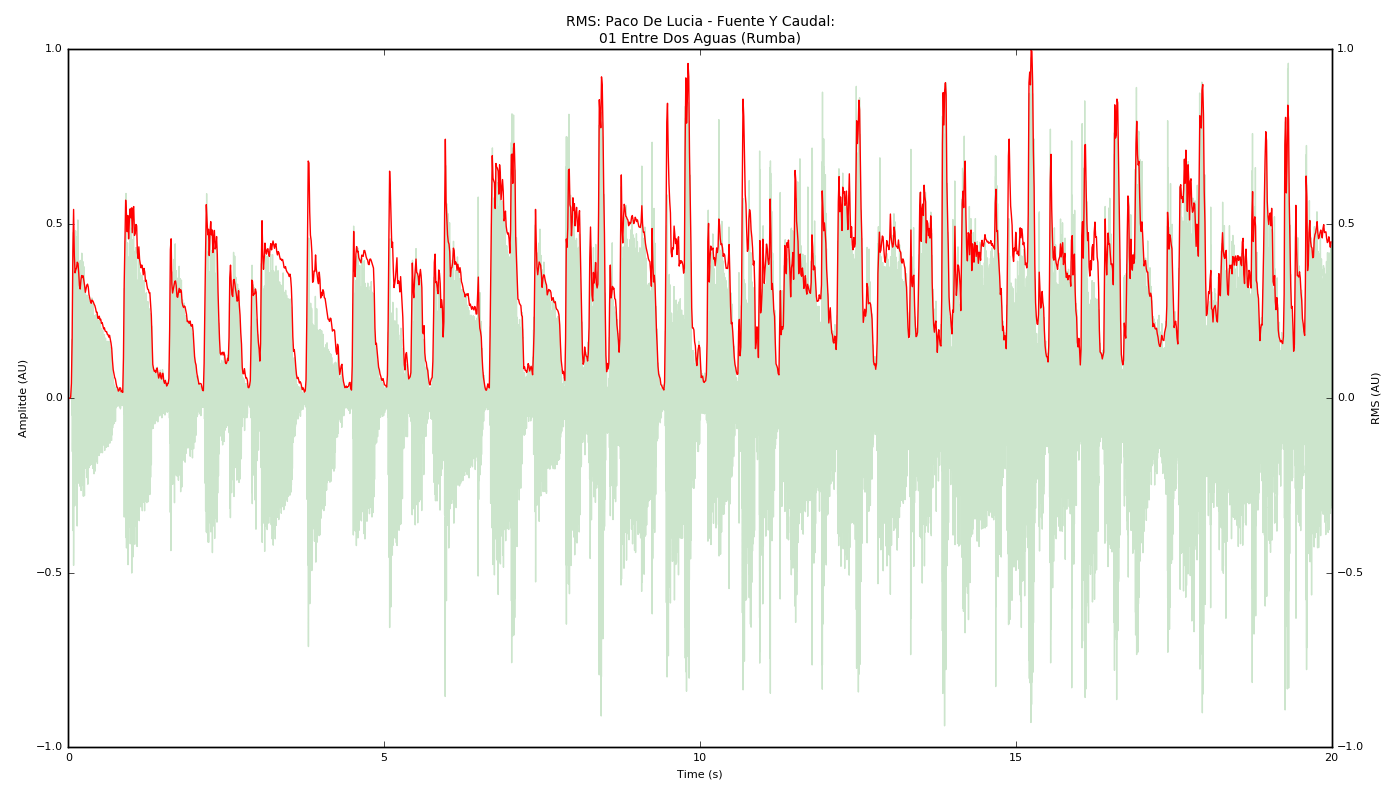
\includegraphics[width=0.75\textwidth]{RMS_Entre_Dos_Aguas.png}
  \caption{RMS superimposed on waveform for the first 20 seconds of a song}
  \label{rms}
\end{figure}

\medskip

\begin{figure}
\centering
  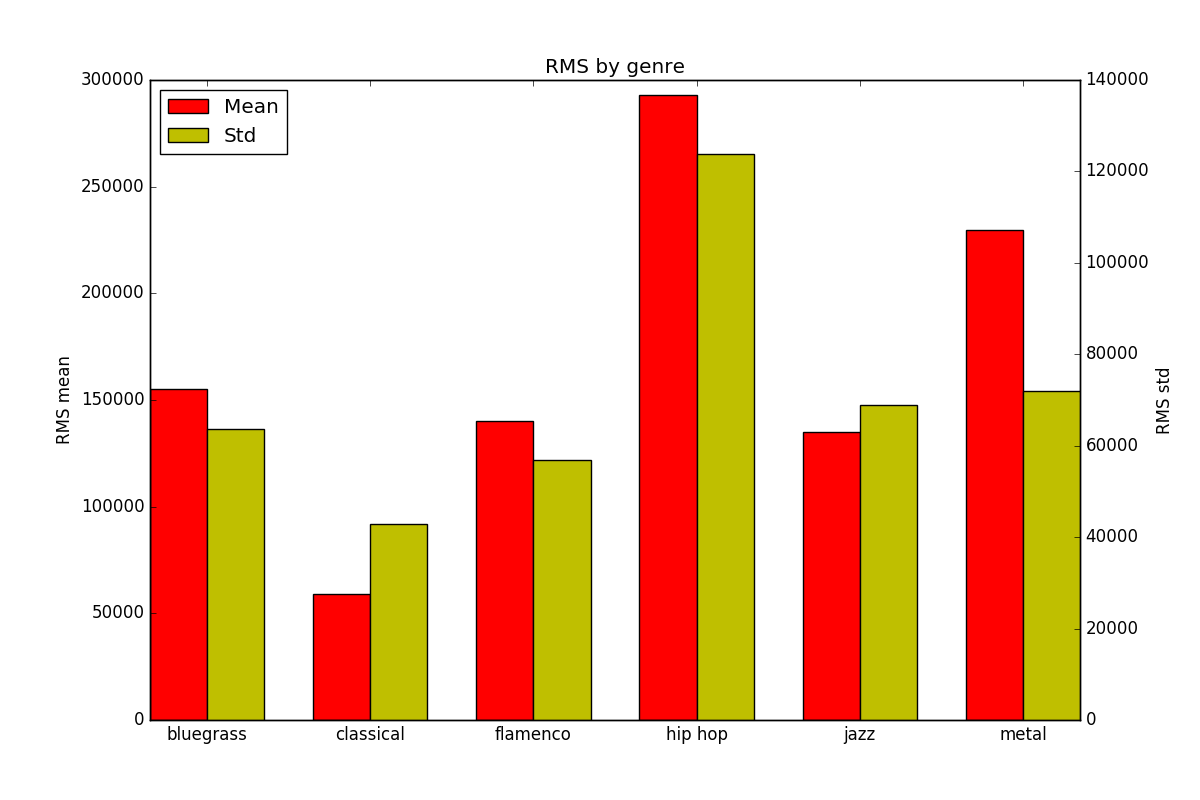
\includegraphics[width=0.75\textwidth]{RMS_by_genre.png}
  \caption{Mean and std of RMS across genres}
  \label{rms_genres}
\end{figure}

\medskip

From figure \ref{rms} we see that the \textit{RMS} actually follows pretty closely our wave, but that is what we would expect since all the \textit{RMS} does is square the amplitudes and then take the square root of the mean. The graph of the variations across genres, as shown in figure \ref{rms_genres} fits our intuition perfectly: we would expect metal and hip hop to be more energetic or loud. We also expect classical to exhibit a relatively larger standard deviation. Once again, this feature is fairly similar in both bluegrass and flamenco which is both exciting (the machine is better at understanding genres than most of us) and worrisome (it may have a hard time differenciating between the two).
\medskip

\subsection*{Frequency domain}
For now we have been concentrating exclusively on features extracted from the time domain, that is, the pure waveform, therefore focusing mostly on amplitude. We would now like to focus our attention on frequency but it is quite hard to study the frequencies from just the waveform. To do that we will make use of the Fourier Transform to go into the frequency domain. The Fourier Transform allows us to jump back and forth between the time and frequency domains. The time domain is simply our waveform, in which we see the evolution of our sound over time, at the expense of specific frequencies information. In the frequency domain we can see the different frequencies, as well as their relative weight, at the expense of time evolution. If we played a pure tone at A4 for a second and then a pure tone an octave higher, A5 for another second the frequency domain would show two sharp peaks, one at 440Hz (corresponding to the A4) and one at 880Hz (corresponding to the A5), but there would be no way of knowing which frequency came first or how long each tone was played for.

To overcome this complete absence of time information in the frequency domain we make use of Short Time Fourier Transform, or STFT. Instead of taking the Fourier Transform of the entire song, the STFT divides the tunes into short windows (in the order of milliseconds) and then takes the Fourier transform of each thus gaining some rich time information. We can then view the result of the STFT in what is called a spectrogram, which conveys the presence, relative strenghts, and evolution of frequencies over time.

\begin{figure}
\centering
  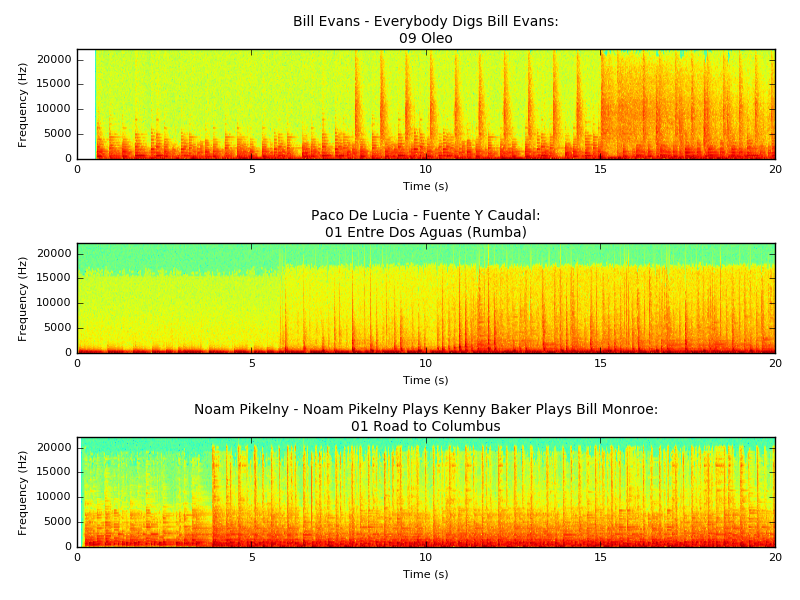
\includegraphics[width=0.75\textwidth]{spectrograms.png}
  \caption{First 20 seconds of three different spectrograms}
  \label{spectrograms}
\end{figure}
 
 \medskip
 
 Let's pause for a second and study these spectrograms one by one. Percussion such as cymbals and snare drums contain a lot of frequencies. In the first tune, Oleo by the Bill Evans trio, the drums come in around second 7 by marking the beat with the cymbals. We can clearly see around ten hits of the hi-hat before the full drums join in around after 15 seconds. The other two tunes both start with a solo instruments. In "Entre dos Aguas" the bass plays the first 5 seconds or so, and we can see that in the spectrogram only low frequencies are preeminent at the beginning. After that the Cajon (a percussion instrument) joins in and we see a lot more frequencies present. The bluegrass song, "Road to Columbus", starts with the banjo. The banjo has a plunky, almost percussive like sound and we can see the difference in timbre and frequencies between the solo bass and solo banjo.
 
\medskip

The power (and beauty) of spectrograms is most striking in classical music. Let us show the full waveform and spectrogram of the prelude to Act III of Richard Wagner's "Meistersinger von Nurnberg". Without even having to listen to the tune we can get an idea of the general colors and loudness from both this graph. Particularly, during the quiet fourth minute we can see the change in color from the deep rich horns to the strings.

\medskip

\begin{figure}
\centering
  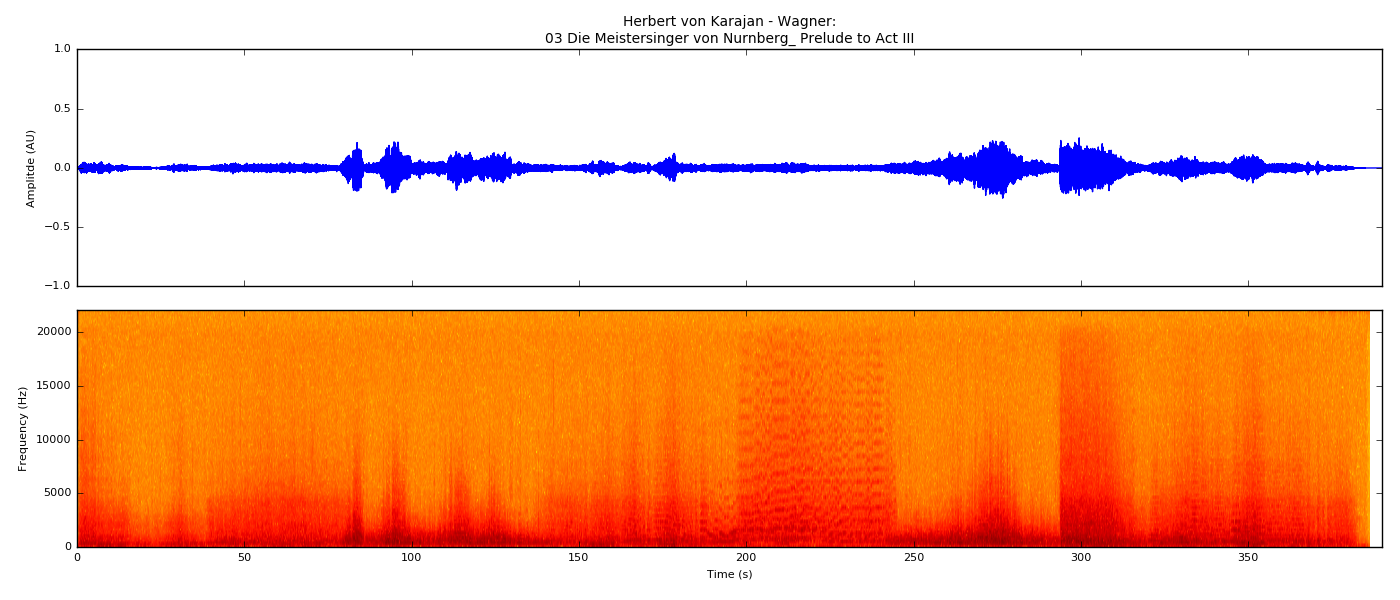
\includegraphics[width=0.75\textwidth]{wagner.png}
  \caption{Full waveform and spectrogram of a classical music piece}
  \label{wave_spec}
\end{figure}

\medskip

Now that we are in the spectral (or frequency) domain, there is a whole new set of features we can extract. We begin by looking at the \textbf{\textit{Spectral Centroid}} or \textit{SC}. Figure \ref{sc} shows the spectral centroid superimposed on the spectrogram for the first 20 seconds of Paco de Lucia's song. The spectral centroid gives us "center of mass" of the spectrum at a specific instant. It translates into the darkness or brightness of sound, with dark having a lower center of mass and bright having a higher one. The first few bass notes of the song have a low spectral centroid. Once all instruments join in, with the guitar and percussion, the spectral centroid takes higher values.

\begin{figure}
\centering
  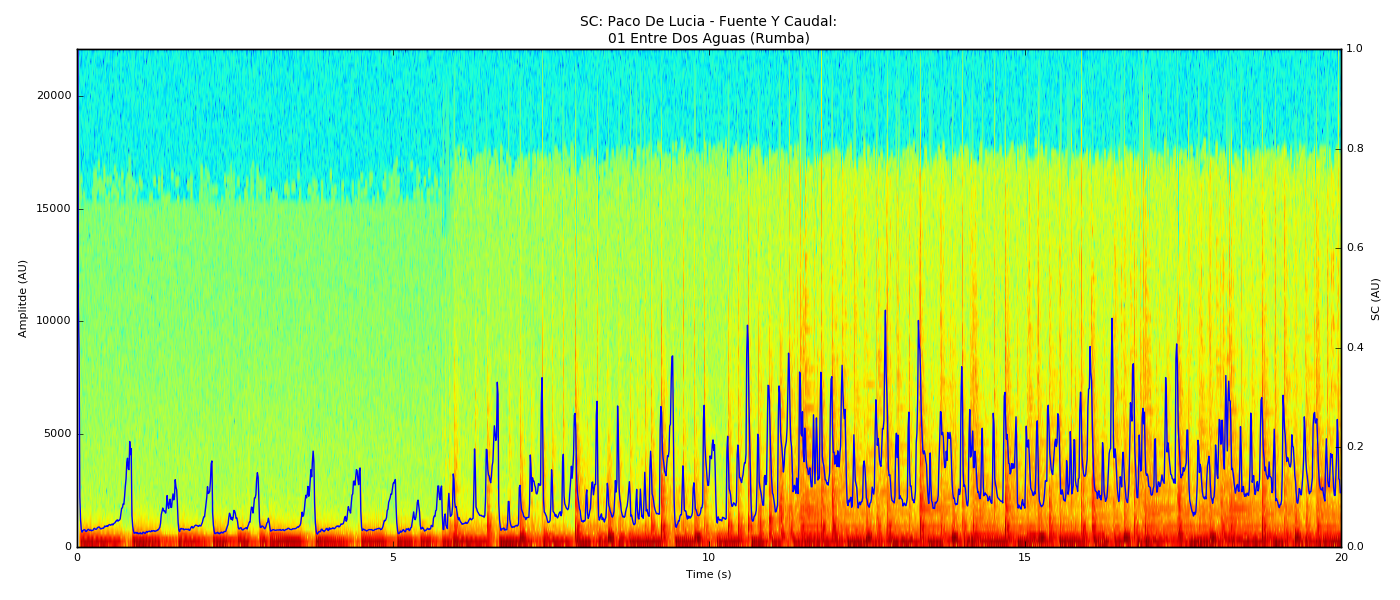
\includegraphics[width=0.75\textwidth]{SC_Entre_Dos_Aguas.png}
  \caption{SC superimposed on spectrogram for the first 20 seconds of a song}
  \label{sc}
\end{figure}

\medskip

Figure \ref{sc_genres} below show the variation of the spectral centroid across genres. As we may expect, jazz (specially Art Blakey, the drummer and band leader chosen as example) is pretty heavy on the cymbals, and the general instrumentation makes the mean value of the spectral centroid pretty high. Once again bluegrass and flamenco have similar values, this time joined by classical music since all three genres have a fuller, darker sound. 


\begin{figure}
\centering
  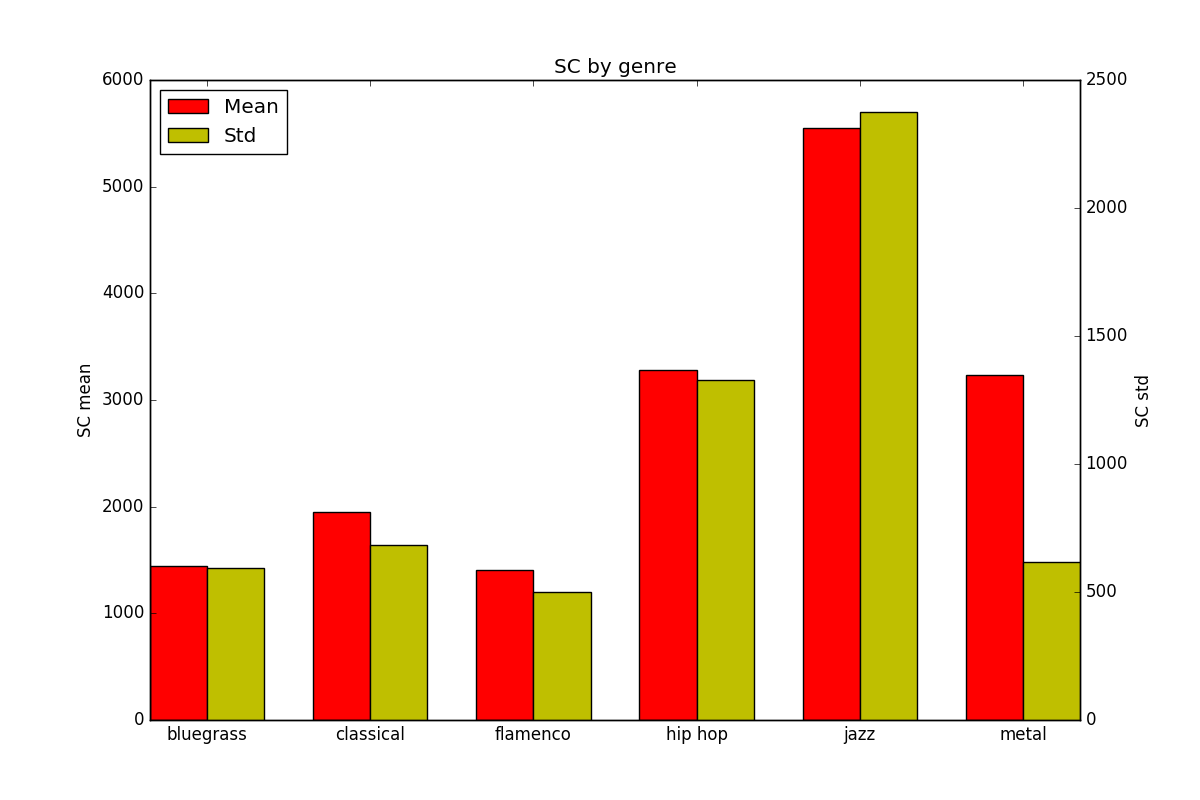
\includegraphics[width=0.75\textwidth]{SC_by_genre.png}
  \caption{Mean and std of SC across genres}
  \label{sc_genres}
\end{figure}

\subsection*{Psychoacoustic features}
We now extract a series of what are called psychoacoustic features. The human auditory system does not exhibit the same sensitivity across all frequencies and thus does not treat all frequencies equally. The Mel scale is a way to properly account for this. The scale is based on human pitch perception. At low frequencies (typically 500Hz) or less, the Mel scale follows linearly the frequency scale. That means that a pitch at double the frequency is perceived by humans as being an octave higher. However as we go past 1000Hz we need increasingly large frequency gaps for humans to perceive a pitch difference. We can say we are more sensitive to low frequencies and less sensitive to higher frequencies. 
\medskip

It is common practice then to split our frequency range into bands, known as Mel bands which are fairly narrow for low frequencies but become larger and larger as we increase the frequency. With this bands we can extract what are known as the \textbf{\textit{Mel Frequency Cepstrum Coefficients }} or \textbf{\textit{MFCC}}. The specific procedure to obtain these coefficients is beyond the scope of this report as it involves switching back and forth between time and frequency domains using "regular" Fourier as well as linear cosine transforms. But broadly speaking we start with the spectrogram, as seen for example in fig \ref{spectrograms}. Then we rescale the y or frequency axis to follow the Mel scale, and split it into the Mel bands. Taking the log of the resulting spectrum and taking what would be another Fourier transform we get a series of coefficients  (typically 13, although the first or zero coefficient contains no relevant information) that show us the evolution of the content of the different Mel bands. We can also study the first order $\Delta$, which represent the frame to frame variation of the coefficients. Figure \ref{mfccs} below show the first 13 MFCCs coefficients along with the first order and second order deltas for Paco de Lucia.

The second order delta is shown for illustrative purposes only, its information content being too low to use it as a relevant feature. We can now take the mean across each of the twelve (we discard the first coefficient) Mel Cepstrum coefficients for both the regular and first order transformation. 
\begin{figure}
\centering
  \includegraphics[width=0.95\textwidth]{MFCCS_Entre_Dos_Aguas.png}
  \caption{MFCC, along with first and second order delta}
  \label{mfccs}
\end{figure}

\medskip

\newpage

\section*{Genre Classification}

Let us recapitulate and review all the features we have extracted. From the time domain we have the \textit{Zero-crossing Rate}, describing the noisiness, and \textit{Root Mean Square} for the loudness. From the frequency domain we have extracted the \textit{Spectral Centroid}, describing the warmth or brightness of our songs. Finally from the spectral domain, but filtered through the Mel frequency banks we have the \textit{Mel Frequency Cepstral Coefficients}, describing the frequency content adjusted for human perception, as well as its first order variations or delta.
\medskip

We have successfully translated sound into something the computer can understand and work with. From tens of millions of integers we have gone to a set of 59 features (we calculate the mean and standard deviation for each feature and included the genre). We are now equipped to begin our exploration of Machine Learning techniques for music.

\subsection*{Preparing the data}
We will start by extracting the features for all songs in our library and saving them in a dataframe and onto memory so that we do not have to extract the features every time we want to try something. For the time being we restrict ourselves for the sake of time to at most the first 5 minutes of each song. For different musical genres the reader may want to use a shorter window and speed things up but because we are using classical music as a genre we need to include as much time as convenience allows to not focus only on the relatively long introductions.
\medskip

The next thing we want to do is get rid of the first MFCC and MFCC $\Delta$ coefficients which convey no useful information. We will also extract the genre labels as a separate dataset, and code them as numbers, with digits 0 to 5 representing genres: bluegrass, classical, flamenco, hip hop, jazz, and metal respectively.

\subsection*{Building the model}
The problem we will try to solve is that of genre classification. Because we have assigned the genres to our songs beforehand by following the filesystem structure proposed this task would fall under supervised learning. Note however that our initial assignment is somewhat arbitrary. That is there are certain flamenco tracks that sound like jazz, but since they belong to a mostly flamenco album they have classified as flamenco. Similarly some jazz may sound like classical and some hip hop like jazz. Because the genres are not deterministic, perfect scores are virtually unachievable.
\medskip

We now split our data into a training and testing set. The training test will be used to train our algorithm and we will use the testing set to test our results. It is common practice in machine learning to perform such a split since the ultimate goal is to be able to make predictions on unseen data. If we used all of the data for training we have a high risk of \textit{overfitting}, that is making our model follow the training data too closely so that predictions on it are almost perfect but the results do not generalize well. Due to the limited amount of data we have (50 songs per genre for a total of 300 songs), we believe a train/test split of 76\%/24\% is appropriate resulting in 228 songs in the training set and  72 in the testing set. Because of the relatively small size of the test set, it is important that each genre is represented more or less equally in the testing set. We therefore choose to perform a stratified shuffle split, which keeps the class ratios in the testing set.
\medskip

Once our data has been split into a training and testing set we can apply one of the most conceptually basic but powerful machine learning algorithms for classification: \textit{K Nearest Neighbors} or \textit{KNN}. \textit{KNN} is a special kind of algorithm in that it does not require any training. It simply stores the data and label in memory and once asked to classify a particular instance, it computes the distance (with a specific distance function) to all points in the training data and assigns a label based on the label of the \textit{K} nearest neighbors. 
\medskip

As a first approach to music genre classification we will apply the "simplest" form of \textit{KNN}, that is without fine-tuning any parameters and using the raw data as our input. We will also look at the $K=1$ case, that is, we only look at the closest point in feature space. Our distance function will be the well known Euclidean distance. 
\medskip

We present our results in the form of a confusion matrix, shown in figure \ref{naiveKNN}. Our confusion matrix consists of six rows and six columns, each representing a genre. The rows represent the true genres and the columns represent the predicted labels. Thus, a song falling into the "Jazz" row, "Classical" column is a Jazz song that was incorrectly classified as Classical.
\medskip
\begin{figure}
\centering
  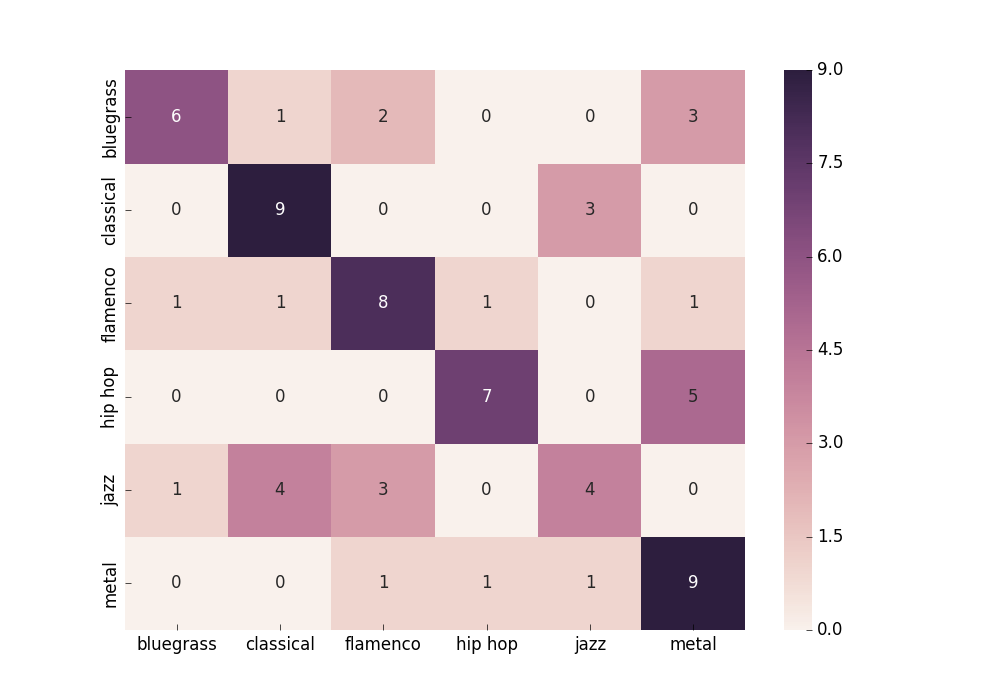
\includegraphics[width=0.95\textwidth]{naiveKNN.png}
  \caption{Confusion matrix for $K=1$ and Euclidean distance}
  \label{naiveKNN}
\end{figure}
\medskip
Before we move to a more quantitative way of measuring performance let's study our results see if they make sense. First of all the results are not bad for a first approach, out of the six different genres we predict four of them accurately more than half the time. We correctly predict nine out of twelve classical and metal songs. This would agree with our understanding of the features being used. Going back to the Music Information Retrieval section, we see that these two genres really stand out from the rest, and even from pure intuition and human perception, these two genres are particularly separate from the rest. We now turn to Jazz, in which our algorithm does not perform so well. We only predict four our twelve songs correctly. The other eight we predict mostly as classical and flamenco. This is not terribly crazy, a quick examination of the songs used to train show that for instance we are using "Peace Piece" by Bill Evans, a very slow, introspective, piano-solo tune that may very well be considered classical music. Another artist featured in our training set is Brad Mehldau, a contemporary pianist who likes to play at the frontiers of jazz, specifically toying with classical music. And then flamenco and jazz artists such as Art Blakey are not that different from a rythmic perspective, both presenting a highly rythmical, asyncopated beat throughout their tunes.
\medskip

We see that our initial approach is not too far off, although it could definitely be improved. But before we do that we look at ways of quantitatively  measure the performance of our model. Some common used metrics are the \textit{precission, recall,} and \textit{F1 score}. All three metrics are defined for each genre in our list. The precision measures the number of instances correctly classified as a particular genre divided the number of songs classified (both correctly and incorrectly) as that genre. Looking at the confusion matrix  we can calculate the precision for each genre by dividing the item in the diagonal by the total number of instances in the column. The recall is similarly defined as the number of instances correctly classified but divided by total number of true instances of that particular genre. So, again, looking at our confusion matrix, we can compute the recall for a genre as the element in the diagonal divided by the total number of songs in the row. Finally the F1 score summarizes both precision and recall in a number from 0 (meaning bad) and 1 according to $F1 = 2*(precision*recall)/(precision+recall)$.

\begin{table}[]
\centering
\begin{tabular}{lrrr}
          & precision & recall & f1 score \\
bluegrass & 0.75      & 0.50   & 0.60     \\
classical & 0.60      & 0.75   & 0.67     \\
flamenco  & 0.57      & 0.67   & 0.62     \\
hip hop   & 0.78      & 0.58   & 0.67     \\
jazz      & 0.50      & 0.33   & 0.40     \\
classical & 0.50      & 0.75   & 0.60     \\
          &           &        &          \\
avg       & 0.62      & 0.60   & 0.59    
\end{tabular}
\caption{Scores of KNN with $K=1$ and Euclidean distance}
\label{naiveKNN_t}
\end{table}
\medskip

What can we compare this numbers against? Let's look at the simplest of baselines which consists of a model which picks a genre at random. What values of precision and recall can we expect from such a model? Since all genres have the same probability of being chosen our each cell on our confusion matrix would (on average) be equally populated. Since we have 72 test set samples and a 6x6 matrix, that means (again, on average) a "2" in each cell leading to a precision, recall and f1 score of 0.166 which incidentally is the probability if selecting a particular genre. Now we have a way of quantitatively measure the performance of our model. In light of these new metric we confirm that our simple model already dramatically outperforms the baseline .
\medskip

\subsection*{Improving the model}
How can we improve our model? The KNN algorithm has a series of parameters we can play with and tune to improve accuracy. The first and most obvious parameter we have available is the number of neighbors \textit{K} used to assign a label. In the previous example we limited ourselves to the most basic case of $K=1$, but we could look at any number of neighbors, varying \textit{K} from one to the number of points in our training set. Another parameter we can tune when considering more than one neighbor is the weighing of the points. When considering  more than one point we can treat them equally, regardless of their distance to the sample we want to classify. Or we could give each neighbor a weight depending on how far it lies on the feature space. And finally we have our distance function. We have a series of distance functions available to us: the well known Euclidean distance, the Manhattan distance (in which the distance is the number of steps taken in the direction of our vector space unit vectors), or the Chebyshev distance (in which the distance is the maximum distance along any one of the vector space directions), for example. However, it is easy to fall into an attitude where we check every single parameter available. There is no reason why Euclidean distance is not appropriate for our setup and we will not explore the other distances available.
\medskip

We perform our exploration of parameter space using grid search. This type of strategy takes a series of possible values for the parameters and a scoring function (in our case the F1 score) and then fits and evaluates a model with each possible combination of parameters, returning the ones that obtain the highest scores. Now, the way we tune this parameter is by looking at the results on the test set. But we may now be at risk of overfitting the testing set with our model parameters! One way out of this is to use cross validation: we first split our data into \textit{k} folds. We then train our model on \textit{k-1} folds and evaluate on the remaining fold, and repeat this procedure for each of different fold groups. After performing our parameter search we obtain that the optimum \textit{K} value is 13 and the weights are to adjusted based on distance. Table \ref{gsKNN_t} summarizes the scores for this new, improved model.

\begin{table}[]
\centering
\begin{tabular}{lrrr}
          & precision & recall & f1 score \\
bluegrass & 0.70      & 0.58   & 0.64     \\
classical & 0.85      & 0.92   & 0.88     \\
flamenco  & 0.82      & 0.75   & 0.78     \\
hip hop   & 0.83      & 0.83   & 0.83     \\
jazz      & 0.50      & 0.50   & 0.50     \\
classical & 0.71      & 0.83   & 0.77     \\
          &           &        &          \\
avg       & 0.74      & 0.74   & 0.73    
\end{tabular}
\caption{Scores of KNN with $K=13$, Euclidean distance, and distance weights}
\label{gsKNN_t}
\end{table}
\medskip

We have significantly improved our model, bringing the overall or average F1 score to 0.73 from the previous 0.59, and improvement can be seen across all genres with the most significant being on jazz and hip hop. Not surprisingly it is this two genres that tend to play more with different styles and so it makes sense that by comparing to a greater collection of neighbors we may more safely classify it than by just looking at the closest neighbors, where songs that lie at the boundary between genres have a greater chance of being misclassified. Our new confusion matrix is shown in figure \ref{gsKNN}.
\begin{figure}
\centering
  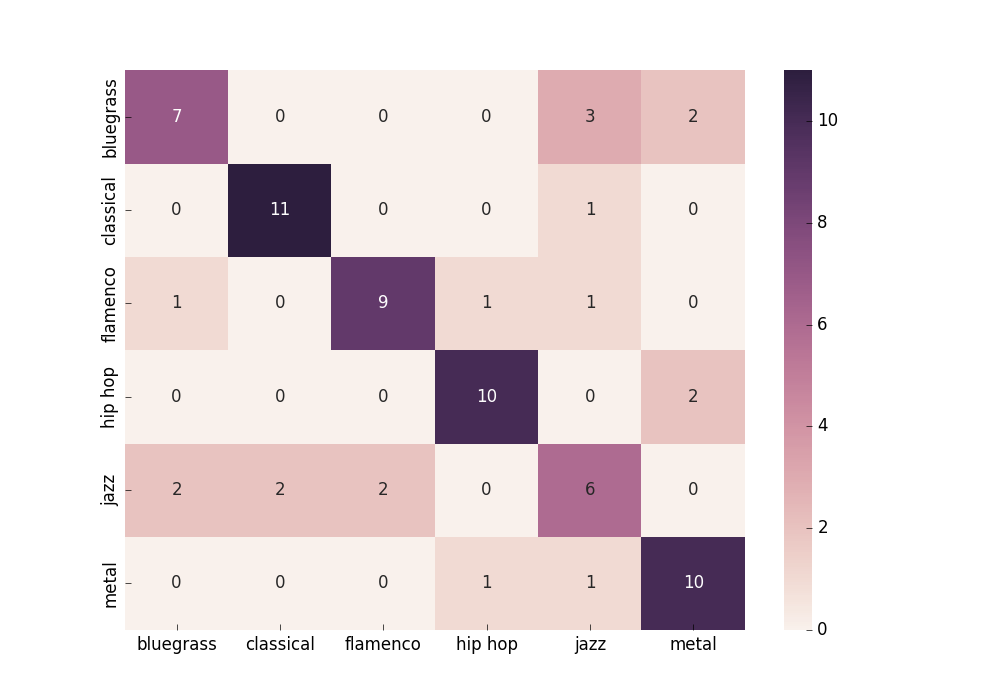
\includegraphics[width=0.95\textwidth]{gsKNN.png}
  \caption{Confusion matrix for $K=13$, Euclidean distance, and distance weights}
  \label{gsKNN}
\end{figure}
\medskip

We have now achieved a fully functional and accurate model. It is able to differentiate correctly between the genres and with precision and recall scores much higher than the baseline. Before we conclude this section and present a simple way to visualize your music library it is worth exploring other models.
\medskip

\subsection*{Exploring alternative models}
An important aspect of the features extracted for our use in this report is that they are not significantly correlated. Of course we can expect loud sections of our audio to contain more frequencies but as figure \ref{wave_spec} showed us, this is not always the case. There is one family of algorithms used for classification whose power and main premise lie in conditional independence between the difference features. Naive Bayes algorithms make use of Bayes rule of probability to make predictions. The simplicity and robustness of this family of algorithms, paired with the data preprocessing performed prior to model training offer great promises for the task of genre classification.
\medskip

Figure \ref{gaussianNB} and table \ref{gaussianNB_t} summarize the results of applying a Gaussian Naive Bayes model to our training set. This simple model clearly outperforms the others, achieving perfect precision and recall in different genres and bringing up the total F1 score all the way up to 0.92

\begin{figure}
\centering
  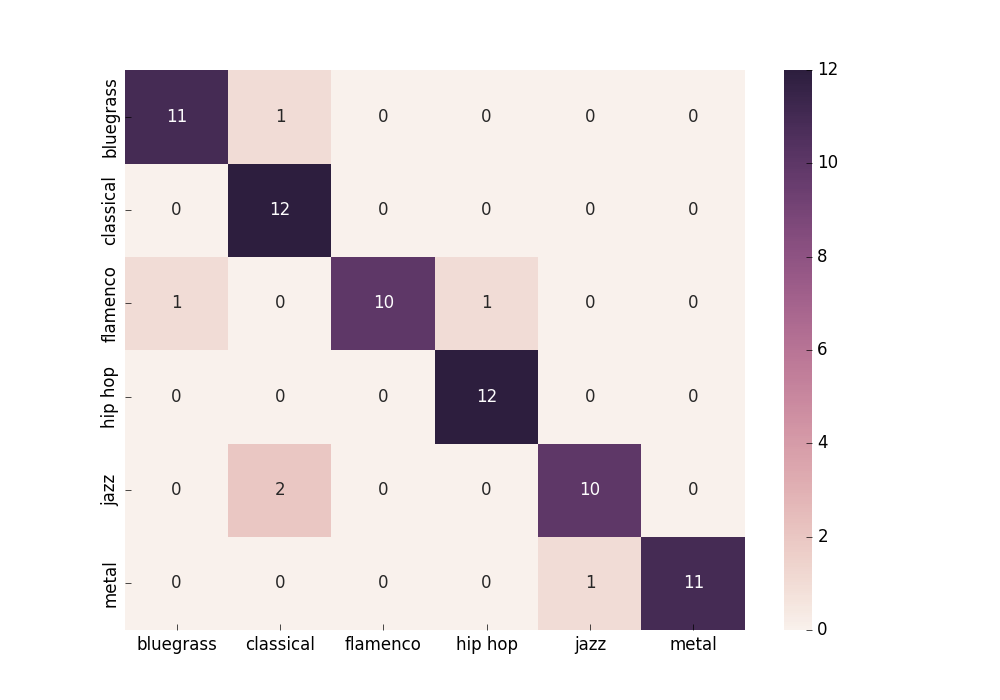
\includegraphics[width=0.95\textwidth]{gaussianNB.png}
  \caption{Gaussian Naive Bayes}
  \label{gaussianNB}
\end{figure}


\medskip
\begin{table}[]
\centering
\begin{tabular}{lrrr}
          & precision & recall & f1 score \\
bluegrass & 0.92      & 0.92   & 0.92     \\
classical & 0.80      & 1.00   & 0.89     \\
flamenco  & 1.00      & 0.83   & 0.91     \\
hip hop   & 0.92      & 1.00   & 0.96     \\
jazz      & 0.91      & 0.83   & 0.87     \\
classical & 1.00      & 0.92   & 0.96     \\
          &           &        &          \\
avg       & 0.92      & 0.92   & 0.92    
\end{tabular}
\caption{Scores of Gaussian Naive Bayes}
\label{gaussianNB_t}
\end{table}
\medskip

\section*{Visualizing your music library}

We conclude this report with a fun way of visualizing your own music library in a two dimensional plane. We recall we have been working in 58 dimensions throughout this report, and the task of visualizing such a space in two dimensions may seem daunting at first. But there is a very powerful dimensionality reduction technique that can accomplish this task, while retaining most of the information.
\medskip

\newpage
\textit{\textbf{Principal Component Analysis}} or \textbf{\textit{PCA}} looks at our data in however many dimensions it lives and changes the coordinate system to follow the directions where data exhibits the most variation. Let's think about what this means with an example: suppose you start off with two dimensional data that lies in an ellipse, but that is not centered or aligned with the axis. The directions of highest variance of the data are of course the major and minor axis of the ellipse. \textit{PCA} moves our original coordinate axis so that our new "x" is aligned with the major axis and our new "y" is along the minor. FIgure \ref{pca_ex} illustrates this procedure.
\medskip

\begin{figure}[ht]
\centering
  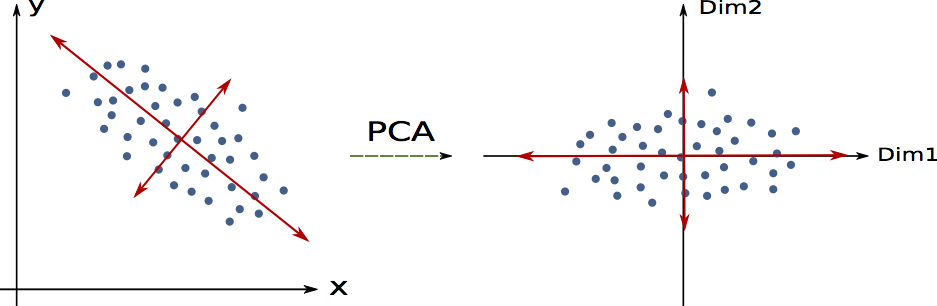
\includegraphics[width=0.75\textwidth]{pca_ex.png}
  \caption{Example of Principal Component Analysis}
  \label{pca_ex}
\end{figure}
\medskip

Before performing PCA analysis on our data, and in order to facilitate interpretation of the PCA components, we manually reduce the dimensions of our data by only considering the \textit{MFCC} means and standard deviations. Since this features relate more closely to our human perception of the sound, while still conveying useful information we consider this set of 26 features to be sufficient to describe and differentiate our genres. We are now in a position to perform PCA on our reduced, 26-dimensional data. Figure \ref{pca_comp} shows the particular linear combination of original dimensions making up our PCA components, as well as the variation in the data explained by each. We see that together the two principal components selected explain $75\%$ of our data.
\begin{figure}
\centering
  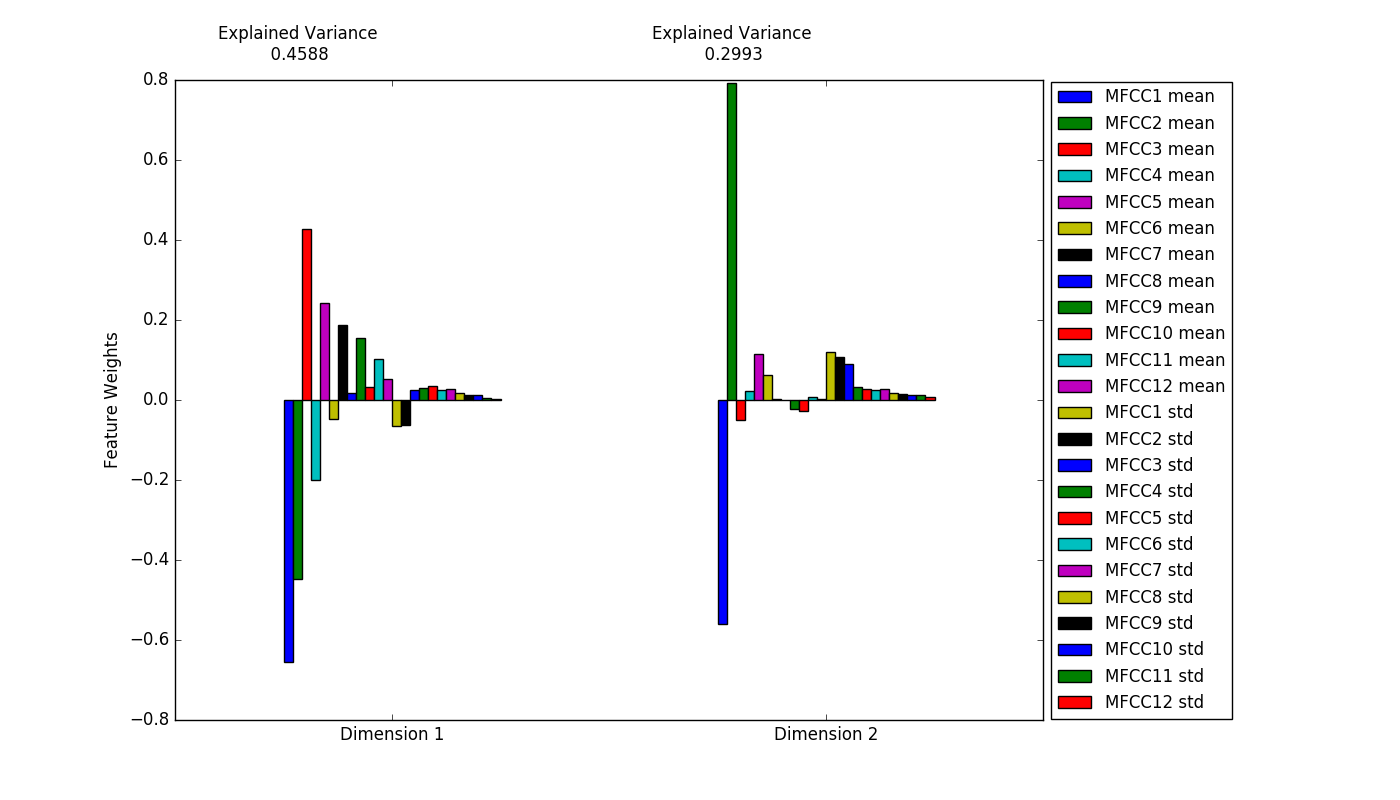
\includegraphics[width=0.9\textwidth]{principal_components.png}
  \caption{Principal Component Analysis on our music data}
  \label{pca_comp}
\end{figure}
\medskip

We can interpret our new dimensions in the light of the relative weight of each\textit{MFCC} in our new dimensions. We recall that the \textit{MFCC} describe the presence and evolution of frequencies in particular bands, these bands being related to our perception of sound. We also recall that the human auditory system has a better sensitivity at relatively low frequencies. We see that our first component reflects songs which carry more weight in the higher frequency bands, at the expense of the first two bands. The same goes for their standard deviations: our first dimension looks for higher variation in the higher frequencies than in our first two bands. Our second component can most easily be described as songs with a very strong presence in the second Mel band, right around where our sensitivity peaks, at the expense of both our first band and higher frequency bands. We thus expect darker and heavier songs to lie towards the bottom left corner while warmer and more percussive (remember percussion has a very rich harmonic spectrum) to lean towards the upper right. Figure \ref{plot_genres} shows our music library plotted along our new axis, colored based on genre.
\begin{figure}
\centering
  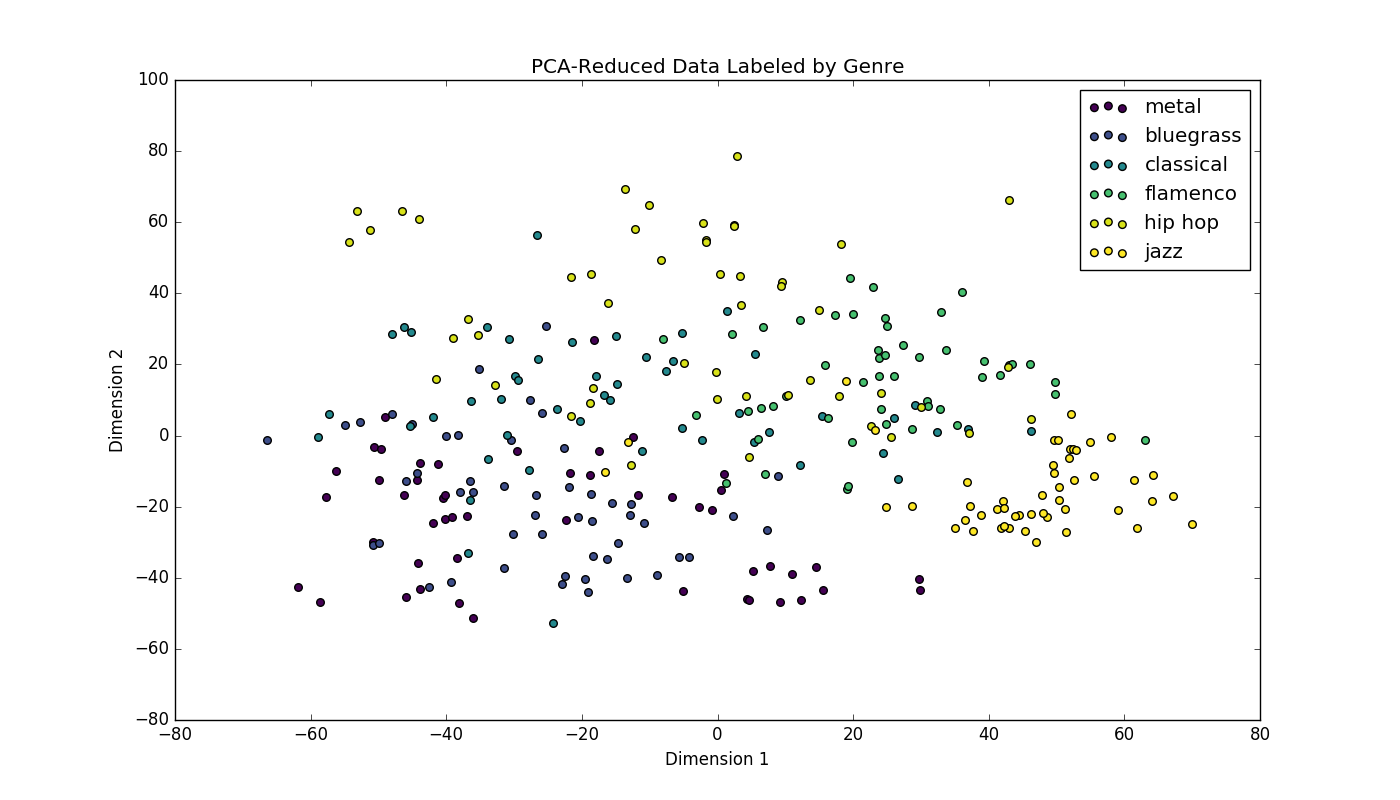
\includegraphics[width=0.9\textwidth]{plot_genres.png}
  \caption{Musical library plotted along PCA components}
  \label{plot_genres}
\end{figure}
\medskip

We do not see clusters as delimited as we would expect from the results of our genre classification but that is natural, after all we have effectively reduced the dimension by a factor of more than 20 and our PCA components only explain 75\% of the variance. We expect our data to form more distinct clusters in higher dimensional space. However we can already confirm visually some of the results obtained during classification. We see, for example that Jazz is much more spread out than other genres with most of the songs clustered to the lower right but some other living in the classical and flamenco spaces. We also see that both classical and metal, our "darker" genres lie in the bottom left, as we would expect.
\medskip

Of course, this graph on its own has little information content, but paired with our genre classification algorithms, it offers a simple and fun way to visualize our music library and to get an rough idea of which genres share more characteristics than others, and which genres lie in opposite sides of the spectrum.
\medskip

\section*{Conclusion}
This short report has offered a glimpse into the complex and fascinating world of music information retrieval, whose task is to extract meaningful features from both the time and frequency domain, as well as psychoacoustic features with the goal of bridging the semantic gap between our understanding of music and the computer's. Features such as \textit{zero-crossing rate, root mean square, spectral centroid}, and \textit{Mel Frequency Cepstral Coefficients} have been explained and extracted.
\medskip

Armed with this new set of features, machine learning techniques have been applied for the task of genre classification. Simple but powerful models such as \textit{K-nearest neighbors} and \textit{Gaussian Naive Bayes} as well of some common metrics to judge the quality of the output of such models have been examined and applied, fine tuning our model parameters using cross-validation.
\medskip

Finally, with the purpose of offering some insights on dimensionality reduction techniques, we have plotted our music library along the dimensions of most variation. This graph offers a simple but attractive way of comparing genres and offers some explanation for the results of our classification models.
\medskip

\newpage
\section*{References}

\begin{itemize}
\item \href{https://www.udacity.com/}{Udacitiy's} Machine Learning Nanodegree material
\item \url{https://github.com/librosa/librosa}
\item \url{http://scikit-learn.org}
\item George Tzanetakis and Georg Essl, "Automatic Musical Genre Classification Of Audio Signals", IEEE Trans on Sp and Audio Proc., 2001
\item \url{http://wwwnew.schindler.eu.com}
\item \url{http://www.ifs.tuwien.ac.at}
\item \url{http://musicinformationretrieval.com/}
\item \url{http://www.christianpeccei.com/musicmap/}
\item \url{http://stackoverflow.com/}
\item Luis Pedro Coelho and Willi Richert, "Building Machine Learning Systems with Python 2 ed.", Packt Publishing, 2015


\end{itemize}








\newpage
\section*{Appendix A: Installations}

The code accompanying this report is built in python 2.7. Below is a list of the different modules and utilities that need to be installed:
\medskip

\begin{itemize}
\item
In order to convert our mp3 or m4a collection to wav from the command line we need \href{https://ffmpeg.org/download.html}{librosa}, along with the mp3 encoder \href{http://lame.sourceforge.net/}{lame}.
\item 
Alternatively, if the our library is exclusively composed of mp3 we can use the faster \href{https://www.mpg123.de/}{mpg123}.

\item
\textbf{Python modules}
\begin{itemize}
\item numpy v1.11.0 for basic algebraic calculations.
\item matplotlib v.1.5.1 for plotting.
\item pandas v.0.18.0 for storing the data in dataframes.
\item librosa v.0.4.3 for music feature extraction.
\item sklearn v.0.17.1 for machine learning.
\item seaborn v0.7.0 for prettier plots.
\end{itemize}
\end{itemize}

\end{document}

%\pyscript{test}{Sample Perl Script With Highlighting}
%
%\begin{center}
%\includegraphics[width=0.75\columnwidth]{example_figure}
%\end{center}
